\documentclass[tikz,border=4pt]{standalone}
\usepackage{amsmath,amssymb}
\usetikzlibrary{arrows.meta,calc,decorations.pathreplacing}
\definecolor{cA}{HTML}{924800}
\definecolor{cB}{HTML}{2F7FC8}
\definecolor{cC}{HTML}{39994B}
\tikzset{
  pt/.style={circle,fill=black,inner sep=0pt,minimum size=4pt},
  disp/.style={-{Stealth[length=2.6mm,width=2mm]},line width=0.9pt,shorten <=2.5pt,shorten >=2.5pt},
  lab/.style={font=\small,sloped,text=black},
  brc/.style={decorate,decoration={brace,amplitude=5pt,raise=3pt},line width=0.6pt},
}
\begin{document}
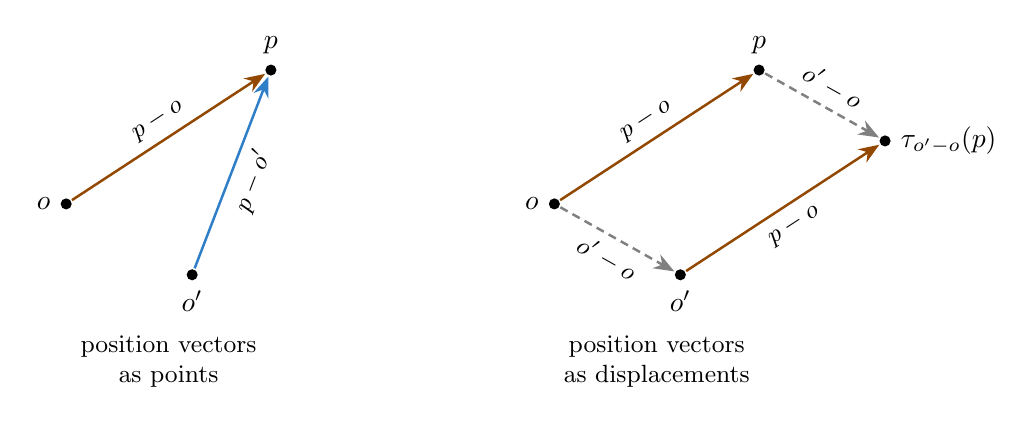
\begin{tikzpicture}
  \coordinate (o) at (0,0); \coordinate (o2) at (1.6,-0.9); \coordinate (p) at (2.6,1.7);
  \draw[disp,cA] (o) -- node[lab,above]{$p-o$} (p);
  \draw[disp,cB] (o2) -- node[lab,below]{$p-o'$} (p);
  \node[pt,label=left:$o$] at (o) {}; \node[pt,label=below:$o'$] at (o2) {}; \node[pt,label=above:$p$] at (p) {};
  \node[font=\small,align=center] at (1.3,-2.0) {position vectors\\as points};
  \begin{scope}[xshift=6.2cm]
    \coordinate (o) at (0,0); \coordinate (o2) at (1.6,-0.9); \coordinate (p) at (2.6,1.7);
    \coordinate (p2) at ($(p)+(o2)-(o)$);
    \draw[disp,gray,densely dashed] (o) -- node[lab,below]{$o'-o$} (o2);
    \draw[disp,gray,densely dashed] (p) -- node[lab,above]{$o'-o$} (p2);
    \draw[disp,cA] (o) -- node[lab,above]{$p-o$} (p);
    \draw[disp,cA] (o2) -- node[lab,below]{$p-o$} (p2);
    \node[pt,label=left:$o$] at (o) {}; \node[pt,label=below:$o'$] at (o2) {};
    \node[pt,label=above:$p$] at (p) {}; \node[pt,label=right:$\tau_{o'-o}(p)$] at (p2) {};
    \node[font=\small,align=center] at (1.3,-2.0) {position vectors\\as displacements};
  \end{scope}
\end{tikzpicture}
\end{document}
